\documentclass[conference,a4paper]{IEEEtran}
\IEEEoverridecommandlockouts
%Template version as of 6/27/2024

\usepackage{cite}
\usepackage{amsmath,amssymb,amsfonts}
\usepackage{graphicx}
\usepackage{textcomp}
\usepackage{xcolor}
\usepackage{booktabs}
\usepackage{multirow}
\usepackage[hidelinks]{hyperref}
\usepackage{array}
\usepackage{xurl}
\def\BibTeX{{\rm B\kern-.05em{\sc i\kern-.025em b}\kern-.08em
    T\kern-.1667em\lower.7ex\hbox{E}\kern-.125emX}}

\title{Quantifying Data Leakage in EEG Emotion Classification: A Four-Tier Evaluation Framework}

\author{\IEEEauthorblockN{Matei-George Sorodoc}
\IEEEauthorblockA{\textit{Dept. of Automation and Applied Informatics} \\
\textit{Technical University of Cluj-Napoca}\\
Cluj-Napoca, Romania \\
sorodoc.a.matei@student.utcluj.ro}
\and
\IEEEauthorblockN{Roxana Rusu Both}
\IEEEauthorblockA{\textit{Dept. of Automation and Applied Informatics} \\
\textit{Technical University of Cluj-Napoca}\\
Cluj-Napoca, Romania \\
roxana.both@campus.utcluj.ro}
}

\begin{document}

\maketitle

\begin{abstract}
EEG-based emotion recognition studies frequently report classification accuracies exceeding 90\% on benchmark datasets, yet these results often rely on evaluation protocols that violate sample independence assumptions. We propose a four-tier evaluation framework that systematically quantifies how evaluation methodology inflates reported performance. The contribution is methodological rather than algorithmic: the framework separates within-trial temporal autocorrelation from cross-subject generalization difficulty and measures each. Using all 32 DEAP subjects and a custom OpenBCI recording (1 subject, 16 channels), both using music-evoked stimuli mapped to Russell's circumplex, we evaluate an MLP baseline and a Graph Attention Network (GAT) under identical conditions for 4-class quadrant and binary classification. Evaluation protocol selection dominates reported performance: 4-class macro F1 degrades from 0.579 (Tier~0, random split) to 0.229 (Tier~2, trial-aware) to 0.178 (Tier~3, LOSO), a 40.1-point drop. Trial leakage ($\Delta=-0.345$, Cohen's $d_z=3.27$, $p<0.001$, $n=32$ subjects) is the dominant inflation mechanism. Once leakage is removed the two architectures are statistically indistinguishable, with confidence intervals spanning zero at Tiers~2 and~3. Binary valence classification yields F1=0.556 under trial-aware evaluation, enabling direct comparison with published benchmarks. On the personalized OpenBCI recording both models exceed 94\% macro F1 under trial-aware evaluation, but control experiments show that this reflects a session confound rather than emotion decoding, indicating that trial-aware evaluation is a necessary but not sufficient standard.
\end{abstract}

\begin{IEEEkeywords}
EEG, emotion recognition, graph attention networks, evaluation methodology, data leakage, brain-computer interface.
\end{IEEEkeywords}

\section{INTRODUCTION}

EEG-based emotion recognition has attracted considerable research attention, with numerous studies reporting classification accuracies between 85--99\% on benchmark datasets such as DEAP~\cite{koelstra2012}. However, many results are obtained using evaluation protocols that inadvertently violate the independence assumption between training and test samples, leading to severely inflated performance estimates~\cite{varoquaux2017, roberts2017}. Recent analyses corroborate this: Khan \textit{et al.}~\cite{khan2025} found that 87\% of 101 reviewed DEAP studies contained methodological errors, including data leakage and biased feature selection, inflating accuracy by up to 46\%, and Lei \textit{et al.}~\cite{lei2025} provided direct empirical evidence that trial-wise leakage inflates EEG emotion classification performance.

The core issue is \emph{trial leakage}: when EEG is segmented into overlapping windows that are then randomly assigned to training and test sets without respecting trial boundaries, near-duplicate feature vectors appear in both, and a classifier can exploit temporal autocorrelation instead of learning emotional representations. Even the moderate 50\% overlap used here produces correlated adjacent windows; the extreme overlaps used elsewhere~\cite{craik2019} worsen this sharply.

This paper contributes a methodology rather than a new model. Prior work has already established that leakage inflates EEG decoding accuracy~\cite{varoquaux2017, khan2025, lei2025}, and we do not claim otherwise. What is new is the systematic decomposition and measurement of that inflation. The four-tier taxonomy separates two mechanisms usually conflated under the single label of data leakage, namely within-trial temporal autocorrelation and cross-subject generalization difficulty, so that a published protocol can be located within the taxonomy and its expected inflation read off. Each mechanism is then quantified on the full 32-subject DEAP corpus for 4-class and binary targets, with effect sizes and confidence intervals reported over an explicitly stated sample unit. The architecture comparison shows that model choice is secondary: once leakage is removed, a graph attention network and a capacity-matched MLP are statistically indistinguishable. We additionally report a personalized single-subject recording as a cautionary case, since it yields near-ceiling accuracy under trial-aware evaluation for reasons that turn out not to be affective.

\section{RELATED WORK}

\subsection{EEG Emotion Recognition}

The DEAP dataset~\cite{koelstra2012} is the most widely used benchmark for EEG emotion recognition: 32 subjects watching 40 one-minute music videos under 32-channel EEG, with self-reported arousal and valence (1--9) as ground truth. Published results vary widely, from 57.5--62.0\% binary accuracy in the original paper to 90--99\% in later deep learning studies~\cite{craik2019}, and that discrepancy is the confound our framework quantifies. Graph-based models have been applied mainly on SEED~\cite{zhong2020, zheng2015} rather than DEAP's arousal-valence formulation, leaving few comparable benchmarks.

Cross-subject generalization has been addressed mainly through architectural or normalization innovations~\cite{fdez2021, li2018ijcai, du2022, ning2021}; Apicella \textit{et al.}~\cite{apicella2024} review 75 such studies and conclude transfer learning is most effective. These works improve the model while holding the protocol fixed, which is the complement of what we vary here.

\subsection{Evaluation Methodology and Our Position}

Leakage in neuroimaging classification is well-documented: improper cross-validation inflates brain decoding accuracy by exploiting temporal structure~\cite{varoquaux2017}, and hierarchically structured data requires CV strategies that respect that dependency~\cite{roberts2017}. Khan \textit{et al.}~\cite{khan2025} and Lei \textit{et al.}~\cite{lei2025} document the problem specifically within the DEAP literature, and EEGain~\cite{kukhilava2025} standardizes preprocessing and splitting across datasets.

Our position should be stated plainly. We are not the first to observe that leakage inflates EEG results, nor do we propose a new splitting algorithm, since Tiers~0 to~3 assemble existing schemes. The contribution is that prior work largely treats leakage as a binary fault, whereas the effect has distinct sources that inflate by different amounts, and an ordered taxonomy makes that inflation attributable.

Graph Attention Networks~\cite{velickovic2018} model EEG channels as graph nodes with attention over channel pairs. Such models report promising within-subject results~\cite{zhong2020} but are rarely examined under cross-trial or cross-subject evaluation, which is the gap our comparison addresses.

\section{METHODOLOGY}

\subsection{Four-Tier Evaluation Protocol}

Windows are 2\,s with 50\% overlap throughout, so a random 80/20 split separates a given pair of adjacent windows with probability $2 \times 0.8 \times 0.2 = 0.32$, making shared signal content exploitable. The four tiers impose progressively stricter constraints on that split. Tier~0 pools all subjects and splits windows randomly 80/20, respecting neither trial nor subject boundaries. Tier~1 runs per-subject 10-fold StratifiedKFold, which removes the cross-subject component but still allows windows from one trial into different folds. Tier~2 runs per-subject StratifiedGroupKFold grouped by trial, so every window of a trial lands in the same fold, and is the minimum standard we advocate. Tier~3 is Leave-One-Subject-Out, training on 31 subjects and testing on the held-out one.

\subsection{DeepGAT Architecture}

DeepGAT treats EEG channels as nodes in a fully-connected $C{\times}C$ graph: 3 GAT layers, 4 heads, dim=96, followed by a dense classifier ($\sim$126K parameters). The MLP baseline flattens the same input and passes it through $C{\times}26 \to 128 \to 64 \to n_c$ ($\sim$116K parameters).

Hyperparameters were optimized using Optuna~\cite{akiba2019} (TPE sampler, 150 trials) with a combined objective: $(\text{F1}_{\text{T1}} + \text{F1}_{\text{T2}} + \text{F1}_{\text{T3}})/3$. Best configuration: lr=$3.9{\times}10^{-3}$, batch=128, label smoothing=0.105, input noise $\sigma$=0.13, attention dropout=0.197.

\subsection{Choice of Architectures}
\label{sec:archchoice}

The two architectures are chosen to isolate one variable, not to survey the design space. Both consume the identical feature tensor at matched capacity ($\sim$116K vs.\ $\sim$126K parameters), so the only difference between them is whether inter-channel relationships are modelled explicitly (GAT) or must be inferred from a flattened vector (MLP). Any gap is therefore attributable to the graph inductive bias rather than to capacity or input representation.

We do not evaluate raw-signal models such as EEGNet~\cite{lawhern2018} or EEG Transformers~\cite{song2023}. This bounds our claims rather than the framework, since the tiers constrain how data is split and are independent of what consumes it. We would expect such models to amplify the effects reported here, because Tiers~0 and~1 reward recognizing that a test window is temporally adjacent to a training window, and a model with direct access to the raw waveform has more signal available for that than one given band-averaged summaries. The prediction is a larger T1 to T2 drop for raw-signal models, testable with the released code.

\subsection{Feature Extraction}

We extract 26 features per channel across five bands: theta (4--8\,Hz), alpha (8--12\,Hz), low beta (12--16\,Hz), high beta (16--25\,Hz) and gamma (25--45\,Hz). These comprise band power (5), differential entropy (5), mean per-channel Phase-Locking Value~\cite{lachaux1999} (5), mean coherence (5), theta-gamma Phase-Amplitude Coupling~\cite{canolty2010} (1) and sub-window band power variability (5). Total dimensionality is $C \times 26$ (832 for DEAP, 416 for OpenBCI), with 2\,s windows at 50\% overlap for both datasets.

\subsection{Datasets}

Both datasets employ music as the emotion-induction stimulus, mapping to Russell's circumplex model of affect~\cite{russell1980}. Holding the stimulus modality constant removes hardware and paradigm differences as explanations for the gap between the two datasets, but it does not make the two label sets equivalent, and Section~\ref{sec:openbci} treats the custom recording accordingly.

We use all 32 DEAP subjects (BioSemi, 32 channels at 128\,Hz, 40 one-minute music-video trials each). Labels derive from self-report arousal and valence via per-subject median splits, forming four quadrants: HAHV, HALV, LAHV, LALV. This convention is standard for DEAP but makes the boundary subject-relative: the arousal median ranges from 1.97 to 7.02 across our subjects, so the same rating can denote high arousal for one participant and low for another. Tiers~0 to~2 are unaffected; Section~\ref{sec:limits} treats the consequence for Tier~3.

The custom OpenBCI recording (Cyton+Daisy, 16 channels at 125\,Hz, one participant, 100 audio trials) is described in full because its structure bounds what can be concluded from it. Tracks were manually selected to target the four quadrants (happy, stressed, calm, sad), 25 per category. Each category was recorded as a single uninterrupted session, its 25 tracks played back-to-back in fixed order, with sessions on different days spanning one day to just under four weeks. The emotion label is therefore perfectly collinear with recording session: no two classes share a session, and no session contains more than one class. The participant was the lead author, who gave informed self-consent. Labels are experimenter-assigned by intended affect, denoting the mood a track was chosen to evoke rather than a verified state.

\subsection{Training Protocol}

All models use AdamW with cosine annealing and class-weighted cross-entropy. Z-score normalization is fit on training data only, per fold, and for LOSO on the $N{-}1$ training subjects, so no feature statistics leak from the test set.

Model selection is also kept off the test fold. Early stopping (patience=20) uses a 15\% validation split carved from the training data alone, and the test fold is used only once, for the reported predictions. This split respects each tier's independence structure, grouped by trial at Tier~2 and by subject at Tier~3, so stopping is judged on the same kind of generalization the tier measures. Selecting the stopping epoch on the test fold would inflate every tier, and the strict tiers most.

\section{RESULTS}

\subsection{What the Reported Statistics Are Computed Over}
\label{sec:statunit}

Because some effect sizes below are large, we state the sample unit explicitly. For Tiers~1 to~3 the unit is the subject: each of the 32 DEAP subjects contributes one macro F1 per tier, itself the mean over that subject's folds (10 for T1 and T2, while for T3 the subject is the fold). Every mean, standard deviation, confidence interval, paired $t$-test and Cohen's $d_z$ for these tiers is computed across those $n=32$ values, paired on subject identity, with 31 degrees of freedom. Fold-level scores are never pooled into the tests, which would inflate $n$ tenfold and understate variance. Tier~0 is the exception, pooling all subjects across 5 random 80/20 splits, so its standard deviation is over splits rather than subjects and is correspondingly small; it serves as an upper-bound reference and is excluded from the paired tests. OpenBCI has one participant, so its unit is the fold.

\subsection{4-Class Quadrant Classification}

Table~\ref{tab:models} presents macro F1 across all tiers. The dominant finding is a 35.0-point F1 drop from T0 to T2 for the GAT, with a further 5.1-point drop to T3.

\begin{table}[t]
\centering
\caption{4-Class Results (DEAP, 32ch, 26 feat/ch, chance = 0.25)}
\label{tab:models}
\begin{tabular}{lcc}
\toprule
Tier & MLP ($\sim$116K) & GAT ($\sim$126K) \\
\midrule
0 (Max leakage) & 0.551 $\pm$ 0.009 & 0.579 $\pm$ 0.006 \\
1 (Within-subj., leaky) & 0.616 $\pm$ 0.104 & 0.574 $\pm$ 0.113 \\
2 (Trial-aware) & 0.234 $\pm$ 0.061 & 0.229 $\pm$ 0.053 \\
3 (LOSO) & 0.171 $\pm$ 0.053 & 0.178 $\pm$ 0.050 \\
\bottomrule
\end{tabular}
\end{table}

The T0 to T1 transition does not move in one consistent direction: MLP rises while GAT is essentially flat, consistent with Tier~1 removing the implicit cross-subject difficulty that pooling introduces at Tier~0, which benefits the stronger leakage-memorizer more. The T1 to T2 transition is the dominant effect for both architectures, identifying trial leakage as the primary inflation source, and the T2 to T3 gap adds cross-subject difficulty on top of it. Paired $t$-tests with Bonferroni correction ($n=32$ subjects) confirm every transition is significant for both architectures: T1 vs.\ T2 ($t=19.2$ MLP, $t=18.5$ GAT, $p<0.001$, $d_z>3.2$) and T2 vs.\ T3 ($t=5.0$ MLP, $t=4.7$ GAT, $p<0.001$, $d_z>0.8$).

Both T2 and T3 fall at or below the nominal 0.25 chance line, so we established that baseline empirically rather than assuming it: with the unbalanced quadrant classes, uniform-random prediction gives a macro F1 of 0.243 and majority-class prediction gives 0.121. Against 0.243, T2 is statistically indistinguishable from chance ($p=0.41$ MLP, $p=0.16$ GAT), whereas T3 falls significantly below it ($t=-7.5$ MLP, $t=-7.3$ GAT, $p<0.001$; 30 and 28 of 32 subjects below chance). Below-chance macro F1 requires systematically biased predictions, and T3 sits between the majority-class and uniform-random baselines, indicating partial collapse onto a subset of classes. Cross-subject transfer therefore does not merely fail, it carries structure that actively misleads, including the subject-relative boundary of Section~\ref{sec:limits}.

\subsection{Architecture Comparison}
\label{sec:archstats}

Testing GAT against MLP with the same subject-paired procedure ($n=32$, Bonferroni-corrected over three tiers) does not support an architectural advantage once leakage is removed. The mean difference in macro F1 is $-0.005$ at T2 (95\% CI $-0.017$ to $+0.007$, $d_z=-0.14$) and $+0.007$ at T3 (95\% CI $-0.013$ to $+0.028$, $d_z=0.13$). Neither is significant, both intervals include zero, and both are far smaller than the tier effects above, by factors of 74 and 7 respectively. The one difference that does survive correction is at T1, where the MLP leads by 0.042 ($d_z=-1.15$, $p<0.001$), consistent with a flat, higher-capacity model exploiting near-duplicate windows more effectively than a spatially structured one. We therefore report the architectures as indistinguishable under trial-aware and cross-subject evaluation, and treat protocol rather than architecture as the operative variable.

\begin{figure*}[!tb]
\centering
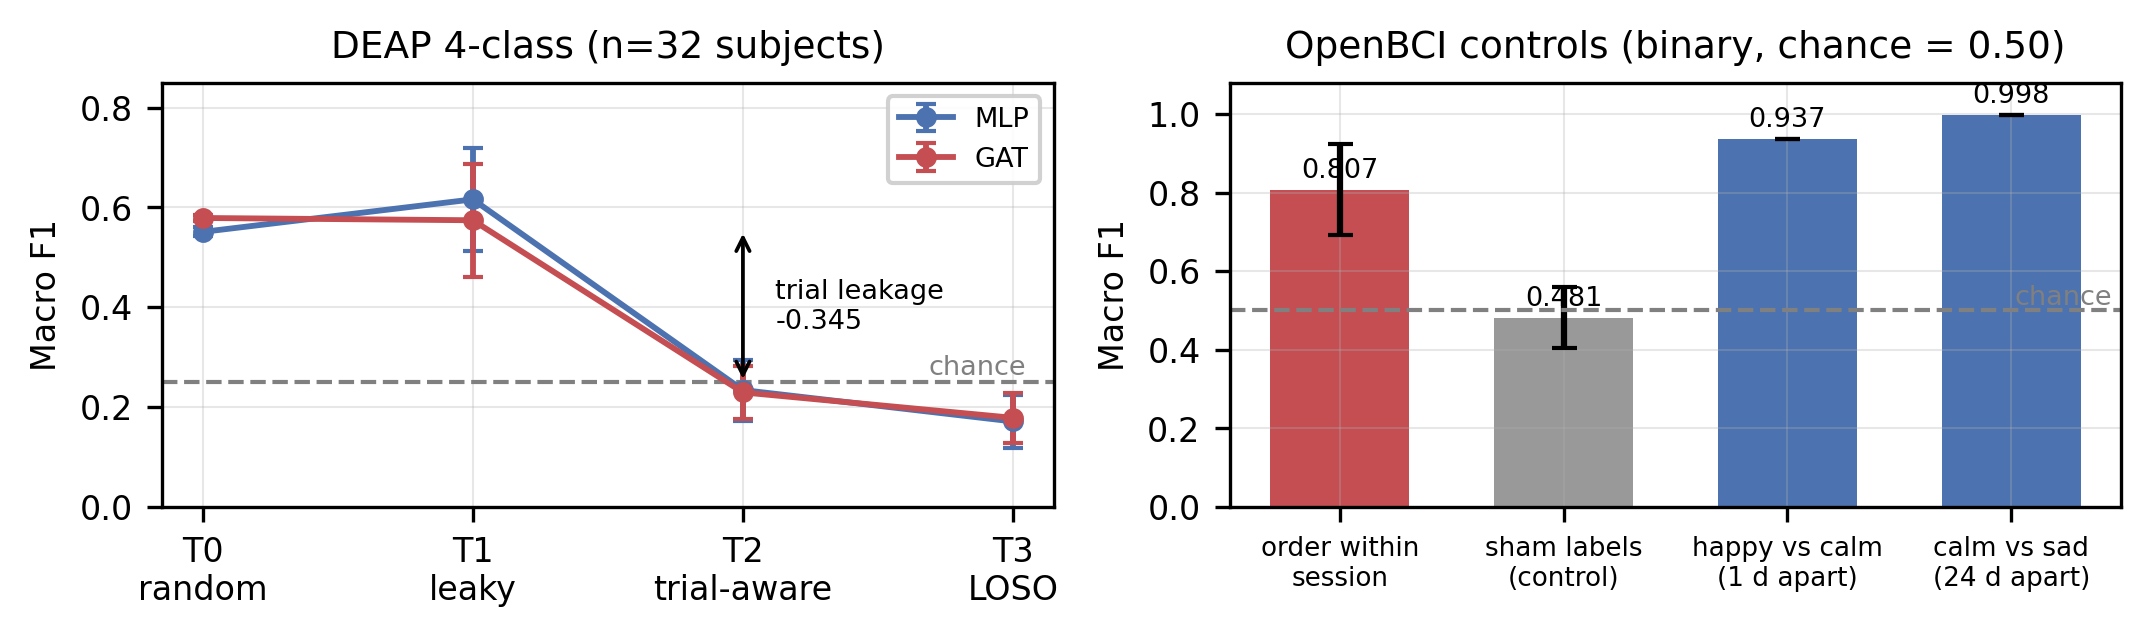
\includegraphics[width=0.92\textwidth]{fig_tier_comparison.png}
\caption{Left: DEAP 4-class macro F1 across the four tiers (chance=0.25). The drop from T1 to T2 identifies trial leakage as the dominant inflation mechanism, and the two architectures track each other throughout. Right: OpenBCI session-confound controls (binary, chance=0.50). Decoding playback order within a single session, holding emotion and day constant, is well above chance, while sham labels stay at chance. The class pair recorded closer in calendar time is not the easier one, contrary to what affective distance would predict.}
\label{fig:degradation}
\end{figure*}

\subsection{Binary Classification}

To contextualize results against the majority of published EEG-BCI literature, Table~\ref{tab:binary} reports binary arousal and valence classification (per-subject median threshold, chance = 50\%). We evaluate the binary task at Tiers~0--2; cross-subject LOSO is reported for the 4-class task, which is the framework's primary demonstration, and repeating it for both binary dimensions would have more than doubled the total compute for a result the 4-class T3 already establishes.

\begin{table}[t]
\centering
\caption{Binary Classification (DEAP, Macro F1, chance = 0.50)}
\label{tab:binary}
\begin{tabular}{llcc}
\toprule
Dim. & Tier & MLP & GAT \\
\midrule
\multirow{3}{*}{Arousal}
 & T0 (random) & 0.676{\scriptsize$\pm$0.005} & 0.678{\scriptsize$\pm$0.005} \\
 & T1 (leaky) & 0.725{\scriptsize$\pm$0.064} & 0.692{\scriptsize$\pm$0.076} \\
 & T2 (trial-aware) & 0.501{\scriptsize$\pm$0.059} & 0.492{\scriptsize$\pm$0.052} \\
\midrule
\multirow{3}{*}{Valence}
 & T0 (random) & 0.716{\scriptsize$\pm$0.009} & 0.717{\scriptsize$\pm$0.005} \\
 & T1 (leaky) & 0.757{\scriptsize$\pm$0.065} & 0.729{\scriptsize$\pm$0.067} \\
 & T2 (trial-aware) & 0.556{\scriptsize$\pm$0.083} & 0.547{\scriptsize$\pm$0.075} \\
\bottomrule
\end{tabular}
\end{table}

The same degradation pattern persists: drops of 18 to 23 points from T1 to T2 confirm that trial leakage inflates binary results substantially. Valence is consistently more discriminable than arousal (0.556 vs.\ 0.501 for MLP at T2), consistent with frontal asymmetry encoding valence more reliably~\cite{allen2004, smith2017}. The architecture verdict matches the 4-class task, with no significant difference at T2 but a significant MLP advantage at T1 in both dimensions ($p<0.001$), the same leakage-memorization signature.

\subsection{The Personalized Recording, and Why Its Accuracy Is Not Emotion Decoding}
\label{sec:openbci}

On the custom OpenBCI dataset (single subject, 100 trials, 16 channels) we evaluate under T0--T2; LOSO is not applicable at $n$=1. Macro F1 is near ceiling throughout: 0.995/0.994 at T0, 0.996/0.995 at T1 and 0.951\,$\pm$\,0.039 / 0.942\,$\pm$\,0.046 at T2 for MLP/GAT respectively.

Trial-aware evaluation barely dents this result, in clear contrast to DEAP, which invites reading it as evidence that emotion decoding becomes tractable once inter-individual variability is removed. Three properties of the acquisition (Section~III-D) make that reading unsafe. Labels are experimenter-assigned, so a correct prediction certifies the track's intended category rather than the participant's state; each class is a fixed set of 25 tracks, so recognizing the stimulus suffices; and each class occupies its own session, so recognizing the session suffices, a session signature such as impedance or cap placement being exactly the slow, spatially structured nuisance a channel-wise spectral pipeline represents well. Trial-aware splitting touches none of these, since all three are constant within a trial and shared across a class.

We ran three controls, using the same protocol, features and models as the headline result, to test whether that nuisance signal is actually decodable rather than merely possible in principle.

Control 1 tests recording order. Within a single session we relabelled trials by playback position, the first 12 tracks against the last 12, and reran the identical protocol. Every window shares the same emotion label, stimulus category and day, so anything above 0.50 is non-affective drift. Macro F1 is 0.807 for MLP and 0.767 for GAT, above chance in all four sessions.

Control 2 is a sham-label check. Repeating Control 1 with trial labels randomly permuted gives 0.481 $\pm$ 0.078 over 20 permutations, confirming that the splitter is not itself leaky and that Control 1 measures real structure.

Control 3 contrasts calendar distance with affective distance. Five of the six one-vs-one problems sit at or above 0.988, so the comparison rests on the one that does not. The happy/calm pair, recorded one day apart, is hardest at 0.937 despite differing in arousal, whereas calm/sad, recorded 24 days apart, separates almost perfectly at 0.998 despite differing only in valence, the opposite of what affective distance predicts. Across all six pairs macro F1 correlates with the calendar gap ($\rho=0.49$ MLP, $0.71$ GAT) and not with circumplex distance ($\rho=-0.41$ and $0.00$). With six pairs and a ceiling effect neither correlation is significant, so this is directional support for Controls 1 and 2 rather than independent evidence.

Control 1 alone is sufficient. A classifier separating the first half of a session from the second at 0.807 does not need emotion to reach 0.95 on four classes recorded on four different days. We therefore do not claim these numbers as evidence for personalized emotion decoding. What the experiment establishes is that trial-aware evaluation is necessary but not sufficient: T2 removes leakage across window boundaries but leaves untouched any nuisance variable constant within a trial and aligned with the label. Where class is confounded with session, T2 reports 0.95 for a model that may have learned no affective representation at all.

\subsection{Computational Cost}
\label{sec:cost}

One complete sweep, covering 4-class at all four tiers plus binary at Tiers~0 to~2 for two architectures and all 32 subjects, took 7.9\,h on a single RTX 3080 with features cached. LOSO should scale worst but converges within roughly 21 epochs, so it proved cheaper than T0 or T1; the larger cost was repeating the sweep for two binary dimensions, which is why we did not extend LOSO to binary. Reporting T1 alongside T2, the minimum we advocate, is inexpensive by comparison.

\section{DISCUSSION}

\subsection{Protocol Dominance Over Architecture}

Evaluation methodology accounts for a 40.1-point F1 variation, from 0.579 at T0 to 0.178 at T3, which is larger than any architectural improvement in the literature. The 34.5-point drop from T1 to T2 dwarfs the MLP-vs-GAT difference at any tier, which never exceeds 4.2 points. This suggests that many published DEAP results reporting above 80\% accuracy operate in what we term the T0/T1 regime, where temporal autocorrelation inflates apparent performance.

The architecture comparison is better stated conservatively. Once trial leakage is removed we cannot distinguish the two architectures on DEAP, since at T2 and T3 the difference between them is small, its confidence interval includes zero, and the paired test does not survive Bonferroni correction (Section~\ref{sec:archstats}). The only effect that does survive runs the other way, with MLP beating GAT at T1, the leaky tier. This is consistent with a flat high-capacity model better memorizing near-duplicate windows, and is therefore a statement about leakage exploitation rather than emotion decoding. Across two architectures with different inductive biases, the spread between them stays an order of magnitude narrower than the spread between protocols.

Residual T2/T3 difficulty plausibly reflects label noise near the median threshold, loss of the shared frequency content exploited at T0/T1, absent domain adaptation, and the 4-class task's difficulty relative to binary.

\subsection{What the Two Datasets Can and Cannot Be Compared On}

Holding stimulus modality constant removes hardware, feature engineering and paradigm as explanations for the DEAP-OpenBCI gap at T2, but does not license attributing it to inter-subject variability alone. The label sets differ in kind, since DEAP records what subjects reported feeling while OpenBCI records what a track was intended to evoke, and Section~\ref{sec:openbci} shows the residual gap is at least partly session identity. Our data cannot establish that calibrated per-user models reach deployable accuracy, since the one personalized corpus available cannot separate that hypothesis from session recognition. Personalized calibration remains reasonable engineering practice~\cite{lotte2018}, but we lack evidence for it here, and would place an acquisition crossing session with label alongside trial-aware splitting as a prerequisite for credible claims.

\subsection{Comparison with Published Results}

Placing published DEAP results in the taxonomy is informative. The original benchmark~\cite{koelstra2012} (57.5--62.0\% accuracy, F1=0.563 binary valence, subject-dependent) sits at approximately T2, and our T2 binary valence of 0.556 lands close to it, consistent with rather than exceeding a benchmark obtained under a comparably rigorous protocol. Studies reporting 90--99\%~\cite{qian2024} use random or trial-leaky splits and belong at T0/T1. Published LOSO baselines on DEAP's arousal-valence formulation are scarce, so our T3 result offers a reference point for cross-subject difficulty.

Several widely cited DEAP studies report 97--100\% under protocols that, per their methods sections, place segments from the same trial in both training and test sets~\cite{algarni2022, chen2019accurate, pichandi2024, jin2020}. We locate these within the taxonomy rather than dispute their implementations; our point is only that such numbers are not comparable to trial-aware ones. That leakage alone can manufacture accuracy is shown by the ``watermelon'' control of Khan \textit{et al.}~\cite{khan2025}: electrodes on an inert watermelon, restructured to mirror DEAP with random labels, reached $>$90\% under segment-level $k$-fold CV while leave-one-trial-out stayed at chance. Where LOSO is applied to DEAP, accuracy falls to 59--72\%~\cite{yang2019}, consistent with our T3 results.

\subsection{Limitations}
\label{sec:limits}

The custom OpenBCI recording is the principal limitation, having one participant, experimenter-assigned labels and a class-per-session design that makes emotion inseparable from session identity. Only a redesigned acquisition, with classes interleaved within session, randomized order, repeated sessions per class and per-trial self-report, could separate them. We report it because the failure mode is common in custom BCI corpora and rarely disclosed.

Tier~3 measures something narrower than cross-subject emotion transfer. Because the quadrant boundary is each subject's own median, the model must transfer a rule defined differently for every training subject, which would depress cross-subject scores even if the neural correlates transferred perfectly, and plausibly contributes to the below-chance result. Our T3 figure is therefore a bound on transfer under the standard DEAP labelling convention rather than a measurement of how well affect generalizes. Separating the two needs a subject-comparable labelling scheme, such as a fixed threshold, which would change the task and its comparability with prior work.

We evaluate two feature-based architectures. Raw-signal models~\cite{lawhern2018, song2023} are outside our scope (Section~\ref{sec:archchoice}), and our expectation of larger leakage effects for them remains untested. Two architectures is a narrow basis, so we state the finding as a negative result: we could not distinguish them, not that no architecture matters. The taxonomy also omits session effects, stimulus-order confounds and label provenance, which the OpenBCI case shows can matter as much. Our PLV and coherence features are also averaged per channel rather than kept as pairwise edge weights, which under-utilizes the graph structure GAT could exploit.

\subsection{Implications for Future Research}

We advocate trial-aware evaluation as the minimum reporting standard, with T1 and T2 both stated so that leakage inflation is quantified rather than assumed absent, and, following Section~\ref{sec:openbci}, with label generation and session structure disclosed for any custom corpus. Beyond protocol, the T2 to T3 gap suggests subject-alignment techniques~\cite{lotte2018, ning2021} as the most promising direction for recovering cross-subject performance, and a neurophysiologically informed adjacency may give the graph inductive bias more to work with than our fully connected one does.

\section{CONCLUSION}

We present a four-tier taxonomy decomposing evaluation-induced inflation into attributable parts, measured on all 32 DEAP subjects. Protocol selection accounts for a 40.1-point macro F1 swing, of which trial leakage is the larger share ($\Delta=-0.345$, $d_z=3.27$, $p<0.001$) and cross-subject difficulty the remainder. Architecture is not distinguishable once leakage is removed, since GAT and a capacity-matched MLP fall within one F1 point at T2 and T3, with paired tests failing to reject equality. Binary valence at T2 (F1=0.556) gives a trial-aware reference point on the task the literature most often reports.

The single-subject recording is a cautionary case rather than a positive result. It reaches 0.95 under trial-aware evaluation, but its labels are collinear with recording session, and controls show non-affective session structure is decodable at 0.807 within one session. The lesson generalizes: trial-aware evaluation is necessary but not sufficient, since it constrains only the window-to-trial relationship and leaves any nuisance variable that is constant within a trial and aligned with the label available to the model. We therefore recommend T2 as the minimum reporting standard, with T1 alongside it so leakage inflation is quantified rather than assumed absent, and with session structure and label provenance of custom corpora disclosed as routine. All code and features: \url{https://github.com/mateisorodoc/Quantifying-Data-Leakage-in-EEG-Emotion-Classification}.

\smallskip\noindent\textit{AI Disclosure:} Claude Opus 4.6 and Gemini 3 Pro were used for language editing and literature search. All scientific content and results are original work by the authors.

\begin{thebibliography}{31}
\setlength{\itemsep}{0pt plus 0.2ex}
\setlength{\parsep}{0pt}

\bibitem{koelstra2012}
S.~Koelstra \emph{et al.}, ``DEAP: A database for emotion analysis using physiological signals,'' \emph{IEEE Trans. Affective Computing}, vol.~3, no.~1, pp.~18--31, 2012.

\bibitem{varoquaux2017}
G.~Varoquaux \emph{et al.}, ``Assessing and tuning brain decoders: Cross-validation, caveats, and guidelines,'' \emph{NeuroImage}, vol.~145, pp.~166--179, 2017.

\bibitem{roberts2017}
D.~R.~Roberts \emph{et al.}, ``Cross-validation strategies for data with temporal, spatial, hierarchical, or phylogenetic structure,'' \emph{Ecography}, vol.~40, no.~8, pp.~913--929, 2017.

\bibitem{khan2025}
N.~N.~Khan \emph{et al.}, ``The role of review process failures in affective state estimation: An empirical investigation of DEAP dataset,'' \emph{arXiv preprint arXiv:2508.02417}, 2025.

\bibitem{lei2025}
P.~Lei, M.~Wu, W.~Yi, and H.~Mo, ``Impact of trial-wise and test data leakage on EEG-based emotion classification,'' \emph{Xidian University preprint}, 2025.

\bibitem{craik2019}
A.~Craik, Y.~He, and J.~L.~Contreras-Vidal, ``Deep learning for electroencephalogram (EEG) classification tasks: A review,'' \emph{J. Neural Engineering}, vol.~16, no.~3, p.~031001, 2019.

\bibitem{zhong2020}
P.~Zhong, D.~Wang, and C.~Miao, ``EEG-based emotion recognition using regularized graph neural networks,'' \emph{IEEE Trans. Affective Computing}, vol.~13, no.~3, pp.~1290--1301, 2020.

\bibitem{zheng2015}
W.-L.~Zheng and B.-L.~Lu, ``Investigating critical frequency bands and channels for EEG-based emotion recognition with deep neural networks,'' \emph{IEEE Trans. Autonomous Mental Development}, vol.~7, no.~3, pp.~162--175, 2015.

\bibitem{fdez2021}
J.~Fdez, N.~Guttenberg, O.~Witkowski, and A.~Pasquali, ``Cross-subject EEG-based emotion recognition through neural networks with stratified normalization,'' \emph{Front. Neurosci.}, vol.~15, p.~626277, 2021.

\bibitem{li2018ijcai}
Y.~Li \emph{et al.}, ``A novel neural network model based on cerebral hemispheric asymmetry for EEG emotion recognition,'' in \emph{Proc. IJCAI}, pp.~1561--1567, 2018.

\bibitem{du2022}
X.~Du \emph{et al.}, ``An efficient LSTM network for emotion recognition from multichannel EEG signals,'' \emph{IEEE Trans. Affective Computing}, vol.~13, no.~3, pp.~1528--1540, 2022.

\bibitem{ning2021}
R.~Ning, C.~L.~P.~Chen, and T.~Zhang, ``Cross-subject EEG emotion recognition using domain adaptive few-shot learning networks,'' in \emph{Proc. IEEE SMC}, pp.~1468--1473, 2021.

\bibitem{apicella2024}
A.~Apicella \emph{et al.}, ``Toward cross-subject and cross-session generalization in EEG-based emotion recognition: Systematic review, taxonomy, and methods,'' \emph{Neurocomputing}, vol.~604, p.~128354, 2024.

\bibitem{kukhilava2025}
N.~Kukhilava \emph{et al.}, ``Evaluation in EEG emotion recognition: State-of-the-art review and unified framework,'' \emph{arXiv preprint arXiv:2505.18175}, 2025.

\bibitem{velickovic2018}
P.~Veli\v{c}kovi\'{c} \emph{et al.}, ``Graph attention networks,'' in \emph{Proc. ICLR}, 2018.

\bibitem{akiba2019}
T.~Akiba \emph{et al.}, ``Optuna: A next-generation hyperparameter optimization framework,'' in \emph{Proc. ACM SIGKDD}, pp.~2623--2631, 2019.

\bibitem{lawhern2018}
V.~J.~Lawhern \emph{et al.}, ``EEGNet: A compact convolutional network for EEG-based brain-computer interfaces,'' \emph{J. Neural Engineering}, vol.~15, no.~6, p.~056013, 2018.

\bibitem{song2023}
Y.~Song, Q.~Zheng, B.~Liu, and X.~Gao, ``EEG Conformer: Convolutional transformer for EEG decoding and visualization,'' \emph{IEEE Trans. Neural Systems and Rehabilitation Engineering}, vol.~31, pp.~710--719, 2023.

\bibitem{lachaux1999}
J.-P.~Lachaux, E.~Rodriguez, J.~Martinerie, and F.~J.~Varela, ``Measuring phase synchrony in brain signals,'' \emph{Human Brain Mapping}, vol.~8, no.~4, pp.~194--208, 1999.

\bibitem{canolty2010}
R.~T.~Canolty and R.~T.~Knight, ``The functional role of cross-frequency coupling,'' \emph{Trends in Cognitive Sciences}, vol.~14, no.~11, pp.~506--515, 2010.

\bibitem{russell1980}
J.~A.~Russell, ``A circumplex model of affect,'' \emph{J. Personality and Social Psychology}, vol.~39, no.~6, pp.~1161--1178, 1980.

\bibitem{allen2004}
J.~J.~B.~Allen, J.~A.~Coan, and M.~Nazarian, ``Issues and assumptions on the road from raw signals to metrics of frontal EEG asymmetry in emotion,'' \emph{Biological Psychology}, vol.~67, no.~1--2, pp.~183--218, 2004.

\bibitem{smith2017}
E.~E.~Smith, S.~J.~Reznik, J.~L.~Stewart, and J.~J.~B.~Allen, ``Assessing and conceptualizing frontal EEG asymmetry: An updated primer on recording, processing, analyzing, and interpreting frontal alpha asymmetry,'' \emph{Int. J. Psychophysiol.}, vol.~111, pp.~98--114, 2017.

\bibitem{lotte2018}
F.~Lotte \emph{et al.}, ``A review of classification algorithms for EEG-based brain-computer interfaces: A 10 year update,'' \emph{J. Neural Engineering}, vol.~15, no.~3, p.~031005, 2018.

\bibitem{qian2024}
R.~Qian \emph{et al.}, ``CSA-SA-CRTNN: A dual-stream adaptive convolutional cyclic hybrid network combining attention mechanisms for EEG emotion recognition,'' \emph{Brain Sciences}, vol.~14, no.~8, p.~817, 2024.

\bibitem{algarni2022}
M.~Algarni \emph{et al.}, ``Deep learning-based approach for emotion recognition using electroencephalography (EEG) signals using bi-directional long short-term memory (Bi-LSTM),'' \emph{Sensors}, vol.~22, no.~8, p.~2976, 2022.

\bibitem{chen2019accurate}
J.~X.~Chen \emph{et al.}, ``Accurate EEG-based emotion recognition on combined features using deep convolutional neural networks,'' \emph{IEEE Access}, vol.~7, pp.~44317--44328, 2019.

\bibitem{pichandi2024}
S.~Pichandi, G.~Balasubramanian, and V.~Chakrapani, ``Hybrid deep models for parallel feature extraction and enhanced emotion state classification,'' \emph{Sci. Rep.}, vol.~14, p.~24549, 2024.

\bibitem{jin2020}
L.~Jin and E.~Y.~Kim, ``Interpretable cross-subject EEG-based emotion recognition using channel-wise features,'' \emph{Sensors}, vol.~20, no.~23, p.~6719, 2020.

\bibitem{yang2019}
F.~Yang \emph{et al.}, ``Multi-method fusion of cross-subject emotion recognition based on high-dimensional EEG features,'' \emph{Front. Comput. Neurosci.}, vol.~13, p.~53, 2019.

\end{thebibliography}

\end{document}
